\chapter{Alloy}

\section{Alloy code}
The following alloy code is created from the class diagram.




\begin{lstlisting}[breaklines=true]
//#SIGNATURES


sig Boolean {
	value : one Int
}
{value=0 or value=1}

sig DateTime{
	timestamp: one Int
}
{timestamp>=0}

abstract sig PaymentMethod{
	valid: one Boolean
}

sig CreditCard extends PaymentMethod{
	expDateID: one DateTime,
}

sig User{
	pmId: one PaymentMethod,
}

sig Transaction{
	userID: one User,
	rentID: one Rent,
	paymMethID: one PaymentMethod,
	amount: one Int
}
{amount > 0}

sig SafeArea{
	carsIn: set Car
}

sig Car{
	rentable: one Boolean,
	inMaintenance: one Boolean,
	inUse: one Boolean,
	reserved: one Boolean,
	inPitStop: one Boolean
}

sig Request {
	carID: one Car,
	userID: one User,
	startTime: one DateTime,
	valid: one Boolean,
	expired: one Boolean
}

sig Rent {
	requestID: one Request,
	costForMinute: one Int,
	systemTimeStart: one DateTime,
	systemTimeEnd: one DateTime,
  	finished: one Boolean
}
{costForMinute > 0}

//#FACTS

fact OneUserOnePaymentMethodValid{
	all u : User | (one pm : PaymentMethod | u.pmId = pm and pm.valid.value = 1)
}

fact ValidRequest{
	all r : Request | r.valid.value = 1 and r.expired.value = 0 iff (one u : User | u = r.userID and one c : Car | c = r.carID)
}

fact NoRequestNotValidButExpired{
	no req : Request | req.valid.value = 0 and req.expired.value = 1
}

fact OneRentOneValidNotExpiredRequest{
	all r : Rent | one req : Request | r.requestID = req and req.valid.value = 1 and req.expired.value = 0
}

fact NoRentWithMoreThanOneRequest{
	no disj r1,r2 : Rent | r1.requestID = r2.requestID
}

fact PaymentOnlyAfterEndRent{
	all r : Rent | r.finished.value = 1 iff (one t1 : Transaction | t1.rentID = r and t1.userID = r.requestID.userID)
}

fact NoTransactionsSameRent{
	no disj t1, t2 : Transaction | t1.rentID = t2.rentID
}

fact RentableCar{
	all c : Car | c.rentable.value = 1 iff (c.inMaintenance.value = 0 and  c.inUse.value = 0 and c.reserved.value = 0 and c.inPitStop.value = 0)
}

fact InMaintenanceCar{
	all c : Car | c.inMaintenance.value = 1 iff (c.rentable.value = 0 and  c.inUse.value = 0 and c.reserved.value = 0 and c.inPitStop.value = 0)
}

fact ReservedCar{
	all c : Car | c.reserved.value = 1 iff (c.rentable.value = 0 and  c.inUse.value = 0 and c.inMaintenance.value = 0 and c.inPitStop.value = 0 and (one r : Request | r.carID = c and r.valid.value = 1 and r.expired.value = 0))
}

fact InUseCar{
	all c : Car | c.inUse.value = 1 iff (c.rentable.value = 0 and  c.reserved.value = 0 and c.inMaintenance.value = 0 and (one r : Request | r.carID = c and r.valid.value = 1 and r.expired.value = 0 and one rent : Rent | rent.requestID = r))
}

fact PitStopOnlyInUseState{
	all c : Car | c.inPitStop.value = 1 implies c.inUse.value = 1
}

fact NoMoreThanOneRequestForCar{
	no disj req1,req2 : Request | req1.carID = req2.carID and req1.valid.value = 1 and req1.expired.value = 0 and req2.valid.value = 1 and req2.expired.value = 0 and
		req2.startTime.timestamp >= req1.startTime.timestamp and req2.startTime.timestamp - req1.startTime.timestamp =< 1
}

fact ReservedCarHasValidRequest{
	all req : Request | (req.valid.value = 1 and req.expired.value = 0) iff (req.carID.reserved.value = 1 or req.carID.inUse.value = 1)
}

fact NoAvailableCarOutSafeArea{
	all c1 : Car | (c1.rentable.value = 1 or  c1.reserved.value = 1) iff (some sa : SafeArea | (one c2 : sa.carsIn | c2 = c1))
}

fact NoSafeAreaWithSameCarIn{
	all c1 : Car |(c1.rentable.value = 1 or c1.reserved.value = 1) implies (no disj sa1, sa2 : SafeArea | c1 in sa1.carsIn and c1 in sa2.carsIn)
}

fact RentNotFinishedCarInUse{
	all r : Rent | r.finished.value = 0 implies	(one c : Car | c = r.requestID.carID and c.inUse.value = 1)
}

fact RentFinishedNotCarInUse{
	all r : Rent | r.finished.value = 1 implies	(one c : Car | c = r.requestID.carID and c.inUse.value = 0)
}

fact PaymentMethodForATransactionAndARent{
	all t : Transaction | (one r : Rent | t.rentID = r and r.finished.value = 1) and (one pm : PaymentMethod | pm.valid.value = 1 and t.paymMethID = pm)
}

fact NoDuplicateDateTime{
	no disj dt1,dt2 : DateTime | dt1.timestamp = dt2.timestamp
}

fact NoDuplicateBoolean{
	no disj b1,b2 : Boolean | b1.value = b2.value
}

//#ASSERTS

assert NoRentWithSameRequest{
	no disj r1,r2 : Rent | r1.requestID = r2.requestID
}
check NoRentWithSameRequest

assert TransactionHasPaymentMethod{
	all t : Transaction | (one r : Rent | t.rentID = r and r.finished.value = 1) and (one pm : PaymentMethod | pm.valid.value = 1 and t.paymMethID = pm)
}
check TransactionHasPaymentMethod


assert CarInUseRentNotFinished{
	all r : Rent | r.finished.value = 0 implies	(one c : Car | c = r.requestID.carID and c.inUse.value = 1)
}
check CarInUseRentNotFinished

assert SafeAreaContainsOnlyCarsReservedOrRentable{
	all c1 : Car | c1.rentable.value = 1 or  c1.reserved.value = 1 iff (one sa : SafeArea | (one c2 : sa.carsIn | c2 = c1))
}
check SafeAreaContainsOnlyCarsReservedOrRentable

assert OneUserOnePaymentMethod{
	all u : User | (one pm : PaymentMethod | u.pmId = pm and pm.valid.value = 1)
}
check OneUserOnePaymentMethod

assert AllRentHasOneValidNotExipredRequest{
	all r : Rent | one req : Request | r.requestID = req and req.valid.value = 1 and req.expired.value = 0
}
check AllRentHasOneValidNotExipredRequest

assert PaymentOnlyAfterEndRent{
	all r : Rent | r.finished.value = 1 iff one t : Transaction | t.rentID = r
}
check PaymentOnlyAfterEndRent

assert CarReservedOnlybyOneRequest{
	no disj req1,req2 : Request | req1.carID = req2.carID and req1.valid.value = 1 and req1.expired.value = 0 and req2.valid.value = 1 and req2.expired.value = 0 and
		req2.startTime.timestamp >= req1.startTime.timestamp and req2.startTime.timestamp - req1.startTime.timestamp =< 1
}
check CarReservedOnlybyOneRequest

assert ReservedCarValidRequest{
	all req : Request | req.valid.value = 1 and req.expired.value = 0 implies req.carID.reserved.value = 1 or req.carID.inUse.value = 1
}
check ReservedCarValidRequest

//#PREDICATES AND SHOWS

pred show1 (){
#Boolean = 2
#Rent = 2
#Transaction = 1
#User = 5
#Car = 4
#Request = 2
#SafeArea = 3
#PaymentMethod = 2

}
run show1 for 10

pred show2 (){
#Boolean = 2
#Rent = 2
#Transaction = 0
#User = 6
#Car = 7
#Request = 3
#SafeArea = 2
#PaymentMethod = 3

}
run show2 for 10

\end{lstlisting}

\section{Alloy generated worlds}
In this section are presented the worlds generated by the alloy analysis software using the given show methods.
\subsection{World 1}
\begin{center}
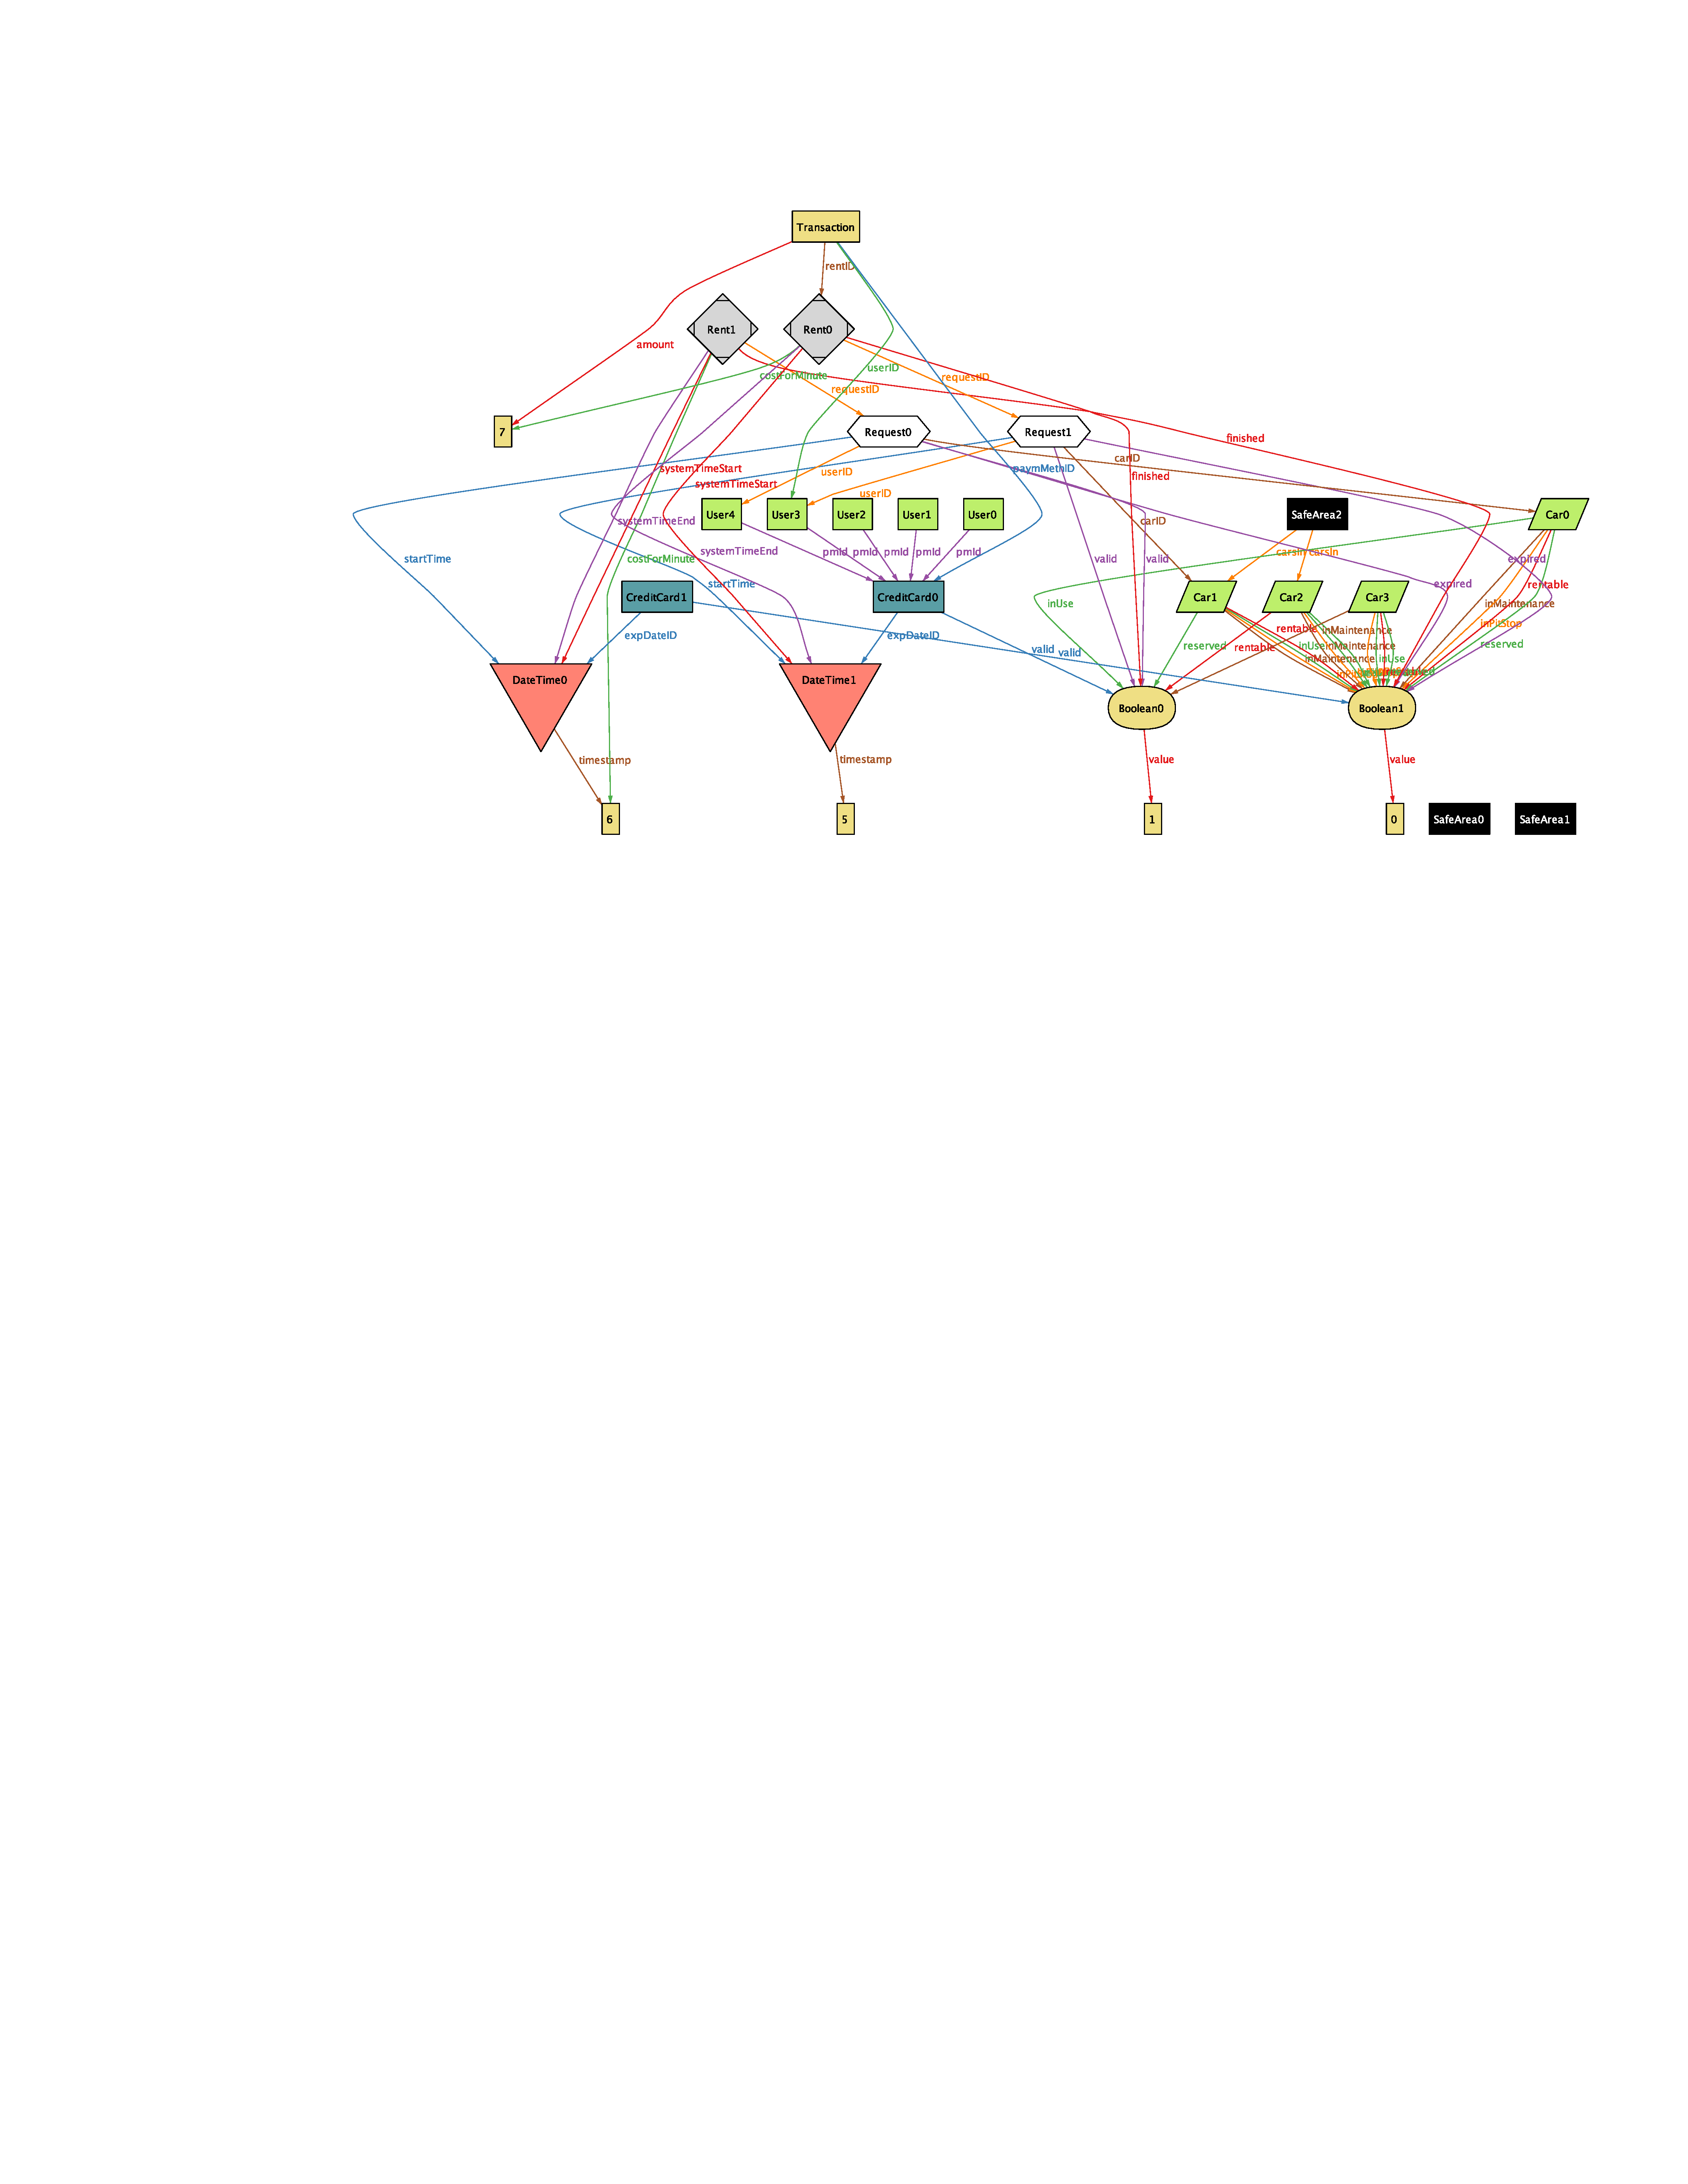
\includegraphics[width=\textheight,keepaspectratio, angle=90]{../images/alloy/world1.pdf}
\end{center}

\subsection{World 2}
\begin{center}
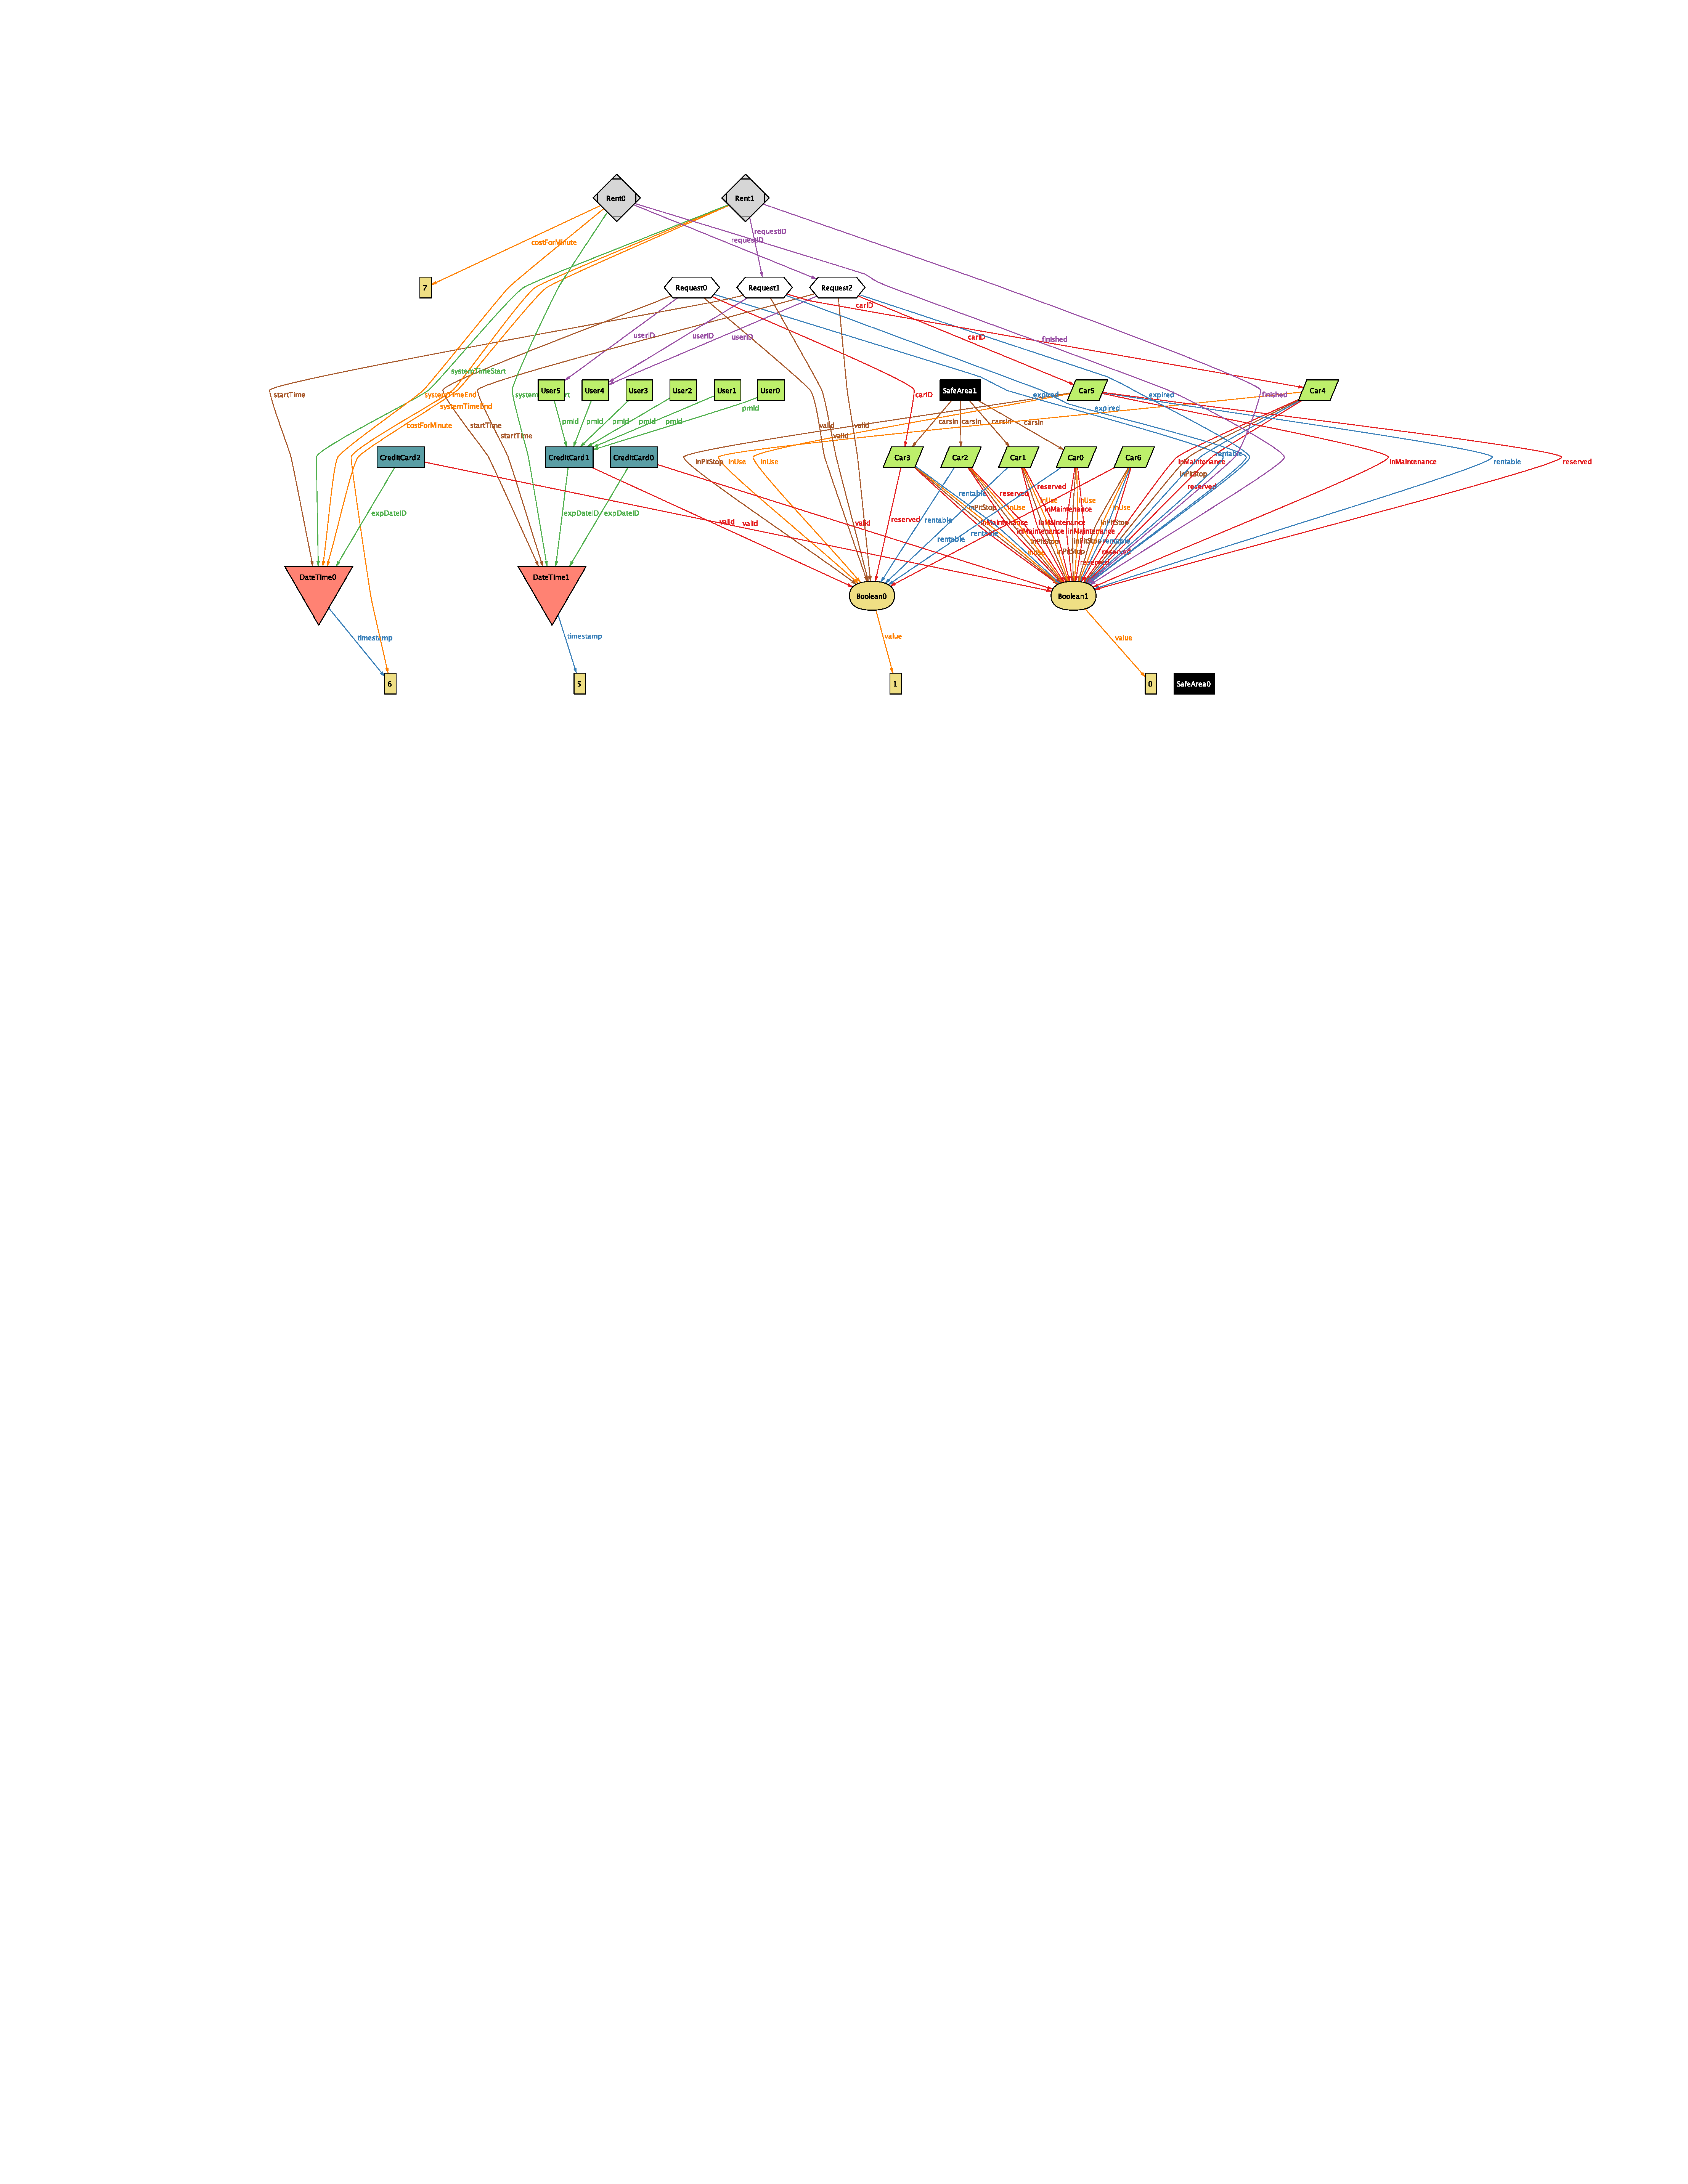
\includegraphics[width=\textheight, keepaspectratio, angle=90]{../images/alloy/world2.pdf}
\end{center}